\let\negmedspace\undefined
\let\negthickspace\undefined
\documentclass[journal]{IEEEtran}
\usepackage[a5paper, margin=10mm, onecolumn]{geometry}
%\usepackage{lmodern} % Ensure lmodern is loaded for pdflatex
\usepackage{tfrupee} % Include tfrupee package

\setlength{\headheight}{1cm} % Set the height of the header box
\setlength{\headsep}{0mm}     % Set the distance between the header box and the top of the text

\usepackage{gvv-book}
\usepackage{gvv}
\usepackage{cite}
\usepackage{amsmath,amssymb,amsfonts,amsthm}
\usepackage{algorithmic}
\usepackage{graphicx}
\usepackage{textcomp}
\usepackage{xcolor}
\usepackage{txfonts}
\usepackage{listings}
\usepackage{enumitem}
\usepackage{mathtools}
\usepackage{gensymb}
\usepackage{comment}
\usepackage[breaklinks=true]{hyperref}
\usepackage{tkz-euclide} 
\usepackage{listings}
% \usepackage{gvv}                                        
\def\inputGnumericTable{}                                 
\usepackage[latin1]{inputenc}                                
\usepackage{color}                                            
\usepackage{array}                                            
\usepackage{longtable}                                       
\usepackage{calc}                                             
\usepackage{multirow}                                         
\usepackage{hhline}                                           
\usepackage{ifthen}                                           
\usepackage{lscape}
\usepackage{circuitikz}
\tikzstyle{block} = [rectangle, draw, fill=blue!20, 
    text width=4em, text centered, rounded corners, minimum height=3em]
\tikzstyle{sum} = [draw, fill=blue!10, circle, minimum size=1cm, node distance=1.5cm]
\tikzstyle{input} = [coordinate]
\tikzstyle{output} = [coordinate]


\begin{document}

\bibliographystyle{IEEEtran}
\vspace{3cm}

\title{2.4.21}
\author{EE25BTECH11026-Harsha}
 \maketitle
% \newpage
% \bigskip
{\let\newpage\relax\maketitle}

\renewcommand{\thefigure}{\theenumi}
\renewcommand{\thetable}{\theenumi}
\setlength{\intextsep}{10pt} % Space between text and floats


\numberwithin{equation}{enumi}
\numberwithin{figure}{enumi}
\renewcommand{\thetable}{\theenumi}

\textbf{Question}:\\
The number of vectors of unit length perpendicular to the vectors $a = 2\hat{i} + \hat{j} + 2\hat{k}$ and $b = \hat{j} + \hat{k} $ is\\ 
\solution \\
Let us solve the given equation theoretically and then verify the solution computationally \\
According to the question,\\
Given the two vectors,
\begin{align}
    \vec{a}=\myvec{2\\1\\2} \;\;\; \vec{b}=\myvec{0\\1\\1}
\end{align}
we need to find the unit vector which is perpendicular to the vectors $\vec{a}$ and $\vec{b}$.The vector perpendicular to $\vec{a}$ and $\vec{b}$ is given by their cross-product.\\
Let the perpendicular vector be $\vec{x}^T=\myvec{x_1&&x_2&&x_3}$
\begin{align}
    \because \vec{a}^T\vec{x}=0\\
    \vec{b}^T\vec{x}=0\;,
\end{align}
\begin{align}
    \therefore \myvec{\vec{a}^T\\\vec{b}^T}\vec{x}=0
\end{align}

\begin{align}
    \myvec{2&&1&&2\\0&&1&&1}\myvec{x_1\\x_2\\x_3}=0
\end{align}
This can be represented as,
\begin{align}
    \myvec{2&&1&&2\\0&&1&&1}
    \xleftrightarrow{\,R_1 \gets R_1-R_2}
    \myvec{2&&0&&1\\0&&1&&1}
\end{align}
yielding,
\begin{align}
    2x_1+x_3=0\\
    x_2+x_3=0
\end{align}
\begin{align}
    \vec{x}=x_3\myvec{\frac{-1}{2}\\-1\\1}=\frac{x_3}{2}\myvec{-1\\-2\\2}
\end{align}

\newpage
\vspace*{0.25cm}
As we know that the vector can be in both the directions i.e, into and out of the plane containing $\vec{a}$ and $\vec{b}$, so the vector perpendicular to vectors $\vec{a}$ and $\vec{b}$ would be $\pm\;(\vec{a} \times \vec{b})$.\\
\\
The desired output is
\begin{align}
    \vec{x}=\pm\frac{1}{3}\myvec{-1\\-2\\2}
\end{align}
\\
From the figure it is clearly verified that the theoretical solution matches with the computational solution.\\
\begin{figure}[H]
    \centering
    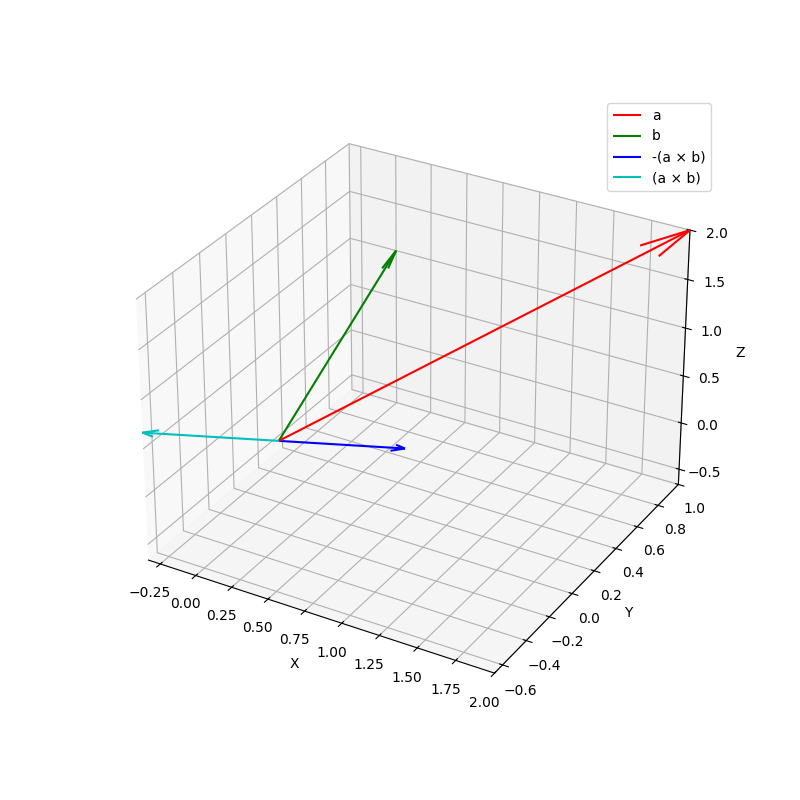
\includegraphics[width=0.8\columnwidth]{figs/Figure_1.png}
    \label{fig-1}
\end{figure}

 


\end{document}
